% ============================================================
% short_paper.tex — Robust Few-shot Image Classification under Label Noise
% 基于 ICLR 2023 workshop 模板（iclr2023_conference.tex）。
%
% 依赖说明：
%   - 需要 iclr2023_conference.sty（官方 ICLR 2023 模板自带；本仓库当前
%     只有主 .tex，请从官方模板包补齐 .sty 文件后即可编译）。
%   - 本文件用内联 thebibliography，无需 .bib / .bst 文件。
%   - 未引入 math_commands.tex 的自定义宏，全部使用标准 amsmath 写法。
%   - 图占位：跑完 run_all.ps1 后取消对应 \includegraphics 行的注释。
% ============================================================
\documentclass{article}
\usepackage{iclr2023_conference,times}
\usepackage{hyperref}
\usepackage{url}
\usepackage{graphicx}
\usepackage{booktabs}
\usepackage{amsmath,amssymb}

\title{Robust Few-shot Image Classification under Label Noise}

% 匿名投稿（ICLR 要求 double-blind，作者信息隐藏）
\author{Anonymous authors\\
Paper under double-blind review}

% 数值结果占位标记：[FILL] 由 run_all.ps1 产出 results/*.csv 后回填
\newcommand{\FILL}{[\textit{FILL}]}

\begin{document}
\maketitle

\begin{abstract}
Few-shot classification assumes a small set of carefully labeled support examples, yet
real-world annotations are frequently noisy. In this paper we study image classification
where each class has only $K$ labeled examples \emph{and} a fraction of those labels are
corrupted. We inject symmetric label noise into CIFAR-10 support sets and show that both a
linear probe trained with cross-entropy and a prototypical network degrade sharply as the
noise rate grows. We propose a simple two-component remedy: (i) \emph{distance-driven sample
selection}, which iteratively trims support examples that lie far from their class
prototype---the few-shot analogue of the ``small-loss'' heuristic---and (ii) a \emph{robust
loss} (Generalized Cross Entropy) applied to the retained examples. Across noise rates of
$0\%$--$40\%$ our method consistently outperforms the baselines on the clean test set, while
the selection step itself doubles as a noise detector. We further analyze which noisy
samples are missed and why, and characterize the resulting prototype drift.
\end{abstract}

\section{Introduction}
\label{sec:intro}

Workshop short papers emphasize a clear research question, a sound experimental design, and
results that support the conclusions. Our question is: \emph{how does label noise interact
with label scarcity, and can a selection-plus-robust-loss method recover clean-test
accuracy?}

Few-shot learners are especially fragile to label noise: with only $K$ examples per class,
a single mislabeled sample already distorts the class prototype, and the distortion grows
with the noise rate. Standard label-noise remedies built for large datasets (large-sample
selection, complex two-stage training) are not directly applicable when the support set is
tiny.

Our contributions are threefold:
\begin{enumerate}
  \item A controlled benchmark injecting symmetric label noise into few-shot support sets
        of CIFAR-10.
  \item A lightweight \emph{distance-driven selection + robust loss} method with an
        interpretable noise-detection signal.
  \item A systematic comparison and ablation across noise rates and few-shot sizes, plus an
        error analysis of misclassification and noise-identification failures.
\end{enumerate}

\section{Related Work}
\label{sec:related}

\textbf{Label-noise robustness.} Methods fall into robust losses (generalized cross entropy
(GCE) \citep{zhang2018gce}, symmetric cross entropy (SCE) \citep{wang2019sce}), sample
reweighting, and sample selection (Co-teaching \citep{han2018coteaching}, DivideMix
\citep{li2020dividemix}). These typically assume thousands of samples per class. We
transplant the \emph{small-loss} idea into prototype space, using \emph{large distance} as
the noisy-sample signal.

\textbf{Few-shot learning.} Prototypical networks \citep{snell2017protonet} classify by
nearest class centroid. When support labels are noisy, the centroid is pulled toward the
wrong class. Prior work on noisy few-shot learning uses meta-learning or label correction;
we show that a simple iterative trimmed prototype plus a robust loss already recovers much
of the accuracy.

\section{Method}
\label{sec:method}

\textbf{Setup.} Given a support set $S = \{(x_i, \tilde{y}_i)\}$ with $N$ classes and $K$
examples per class, where labels $\tilde{y}$ are corrupted by symmetric noise at rate $r$.
A frozen ImageNet-pretrained ResNet-18 extracts L2-normalized features $f(x_i)$. A clean
test set is used only for evaluation.

\textbf{Baselines.}
\begin{itemize}
  \item \emph{ProtoNet}: prototype $p_c = \frac{1}{|\{i:\tilde{y}_i=c\}|}\sum_{i:\tilde{y}_i=c} f(x_i)$,
        classify by cosine similarity.
  \item \emph{CE linear probe}: a linear head trained on $(f(x_i), \tilde{y}_i)$ with
        cross-entropy.
\end{itemize}

\textbf{Component 1 --- distance-driven selection.} We compute prototypes, then measure
each support sample's distance to \emph{its (possibly wrong) assigned class prototype}. A
sample is flagged as noise if its distance exceeds a threshold
\[
  d_i = 1 - \cos\bigl(f(x_i),\, p_{\tilde{y}_i}\bigr) > \mu + \beta\,\sigma,
\]
where $\mu,\sigma$ are the mean and standard deviation of the within-set distances, or
alternatively via a fixed quantile $\tau$. Prototypes are then recomputed from the retained
samples, and we iterate $T$ rounds. This is the prototype-space translation of ``small loss
= clean.''

\textbf{Component 2 --- robust loss.} We train a linear head on the retained samples using
GCE
\[
  \mathcal{L}_{\mathrm{GCE}} = \frac{1 - p_{y}^{q}}{q},
\]
which is bounded for mislabeled examples and thus robust to residual noise that selection
misses.

\textbf{Variants for ablation:} selection-only, robust-loss-only, and full (both).

\section{Experiments}
\label{sec:experiments}

\textbf{Setup.} CIFAR-10; $N=10$ classes; $K \in \{5,10,20\}$; symmetric noise
$r \in \{0, 0.1, 0.2, 0.4\}$; frozen ResNet-18 (ImageNet) features, 512-d, L2-normalized.
Metrics: accuracy, macro-F1, ECE (15 bins), and noise-detection precision/recall/F1. Seeds
fixed; noise mask and configs saved for reproducibility.

\textbf{Results.} Table~\ref{tab:acc} reports clean-test accuracy versus noise rate at
$K=10$, and Table~\ref{tab:noise} reports the noise-detection quality of the selection step.

\begin{table}[t]
  \centering
  \caption{Clean-test accuracy (\%) vs.\ label noise rate ($K=10$, CIFAR-10).}
  \label{tab:acc}
  \begin{tabular}{lcccc}
    \toprule
    Method           & 0\%  & 10\% & 20\% & 40\% \\
    \midrule
    ProtoNet         & \FILL & \FILL & \FILL & \FILL \\
    CE linear probe  & \FILL & \FILL & \FILL & \FILL \\
    selection-only   & \FILL & \FILL & \FILL & \FILL \\
    robust-loss-only & \FILL & \FILL & \FILL & \FILL \\
    \textbf{full}    & \FILL & \FILL & \FILL & \FILL \\
    \bottomrule
  \end{tabular}
\end{table}

\begin{table}[t]
  \centering
  \caption{Noise-detection precision / recall / F1 of the selection step (full method).}
  \label{tab:noise}
  \begin{tabular}{lccc}
    \toprule
    Method & 10\% & 20\% & 40\% \\
    \midrule
    full   & \FILL & \FILL & \FILL \\
    \bottomrule
  \end{tabular}
\end{table}

\emph{Expected finding}: full $>$ each single component $>$ CE baseline; the gap widens with
noise rate. ECE and macro-F1 follow the same trend. Calibration degrades with noise (higher
ECE), and our method partially restores it.

\textbf{Ablations.} Sweep $\beta$, $q$, $T$, and the $\tau$ variant at $r=0.4$ (see
\texttt{results/ablation\_summary.csv}). \emph{Expected}: moderate $\beta$ and
$q\approx0.7$ are stable; very aggressive trimming (small $\beta$/$\tau$) over-fits but
hurts recall of clean samples.

\textbf{Few-shot scale.} At $r=0.4$, sweep $K \in \{5,10,20\}$. \emph{Expected}: the benefit
of our method is largest at the smallest $K$, where each sample matters most.

\begin{figure}[t]
  \centering
  % 跑完 run_all.ps1 后取消注释：
  % 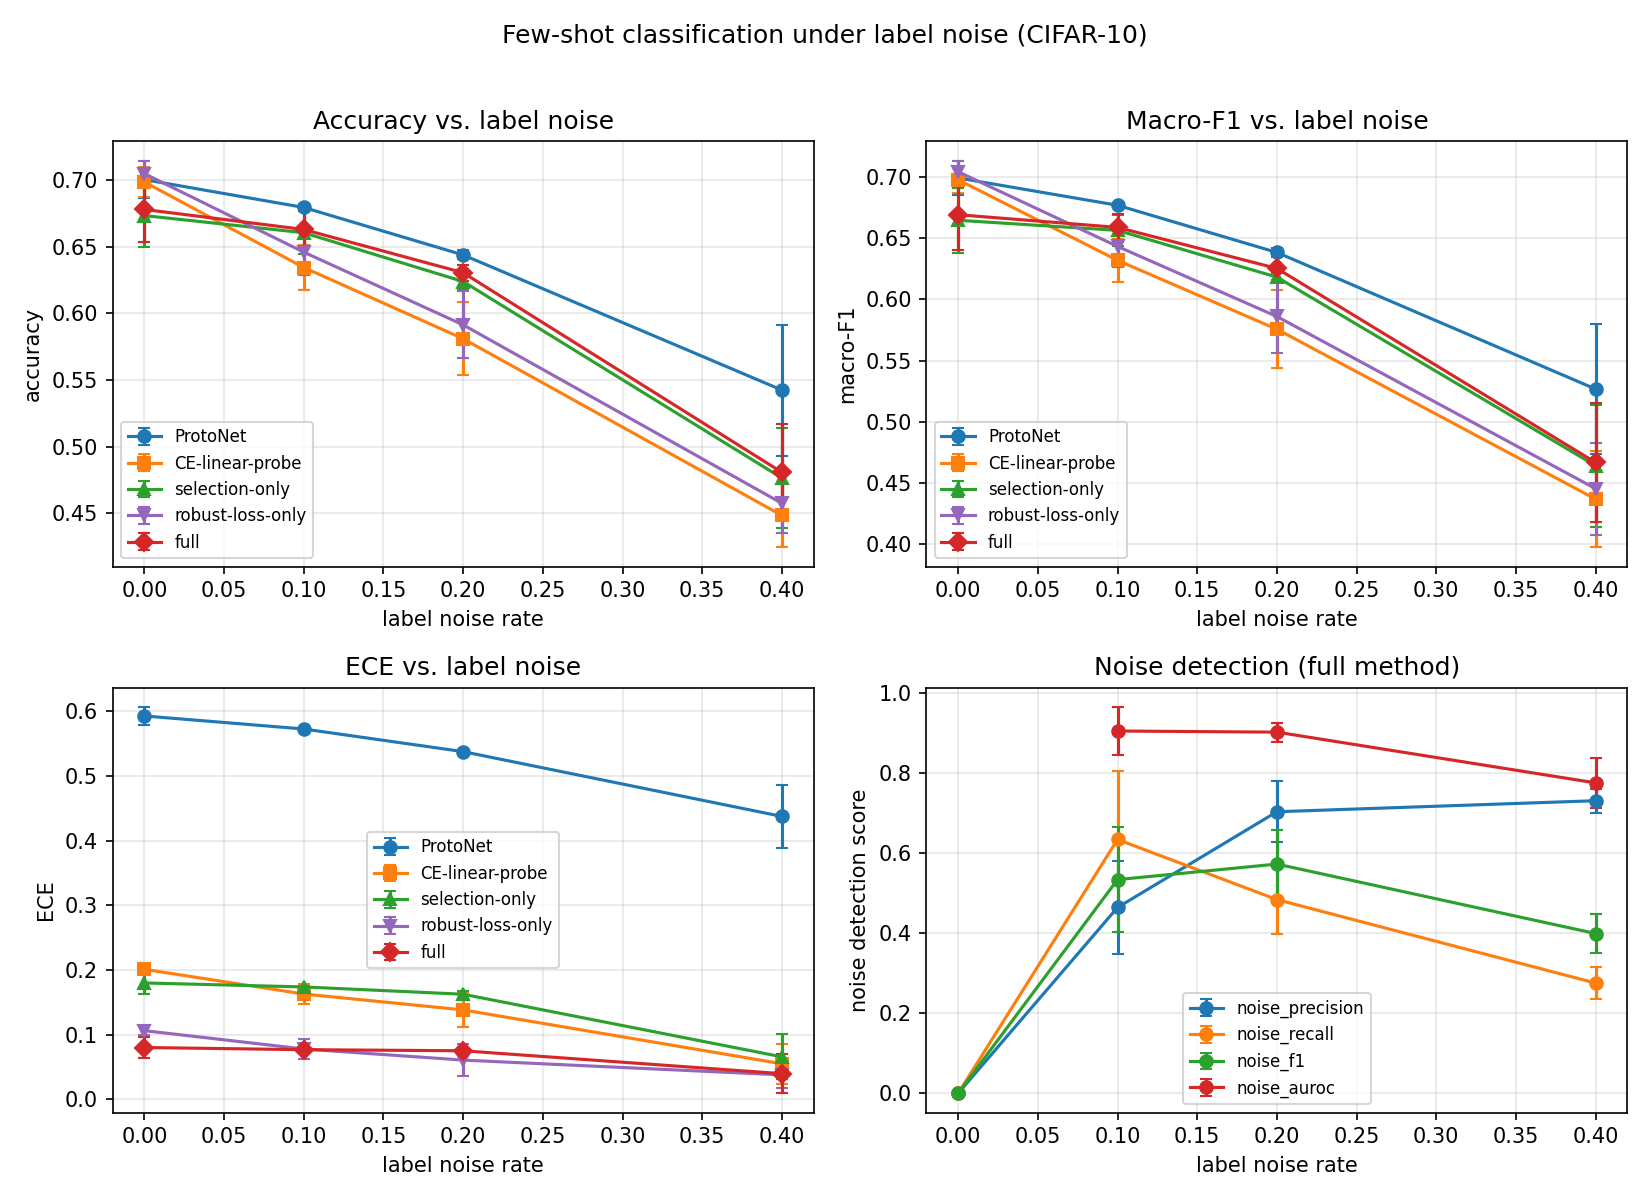
\includegraphics[width=0.95\linewidth]{../results/figs/main_results.png}
  \caption{Accuracy, macro-F1, and ECE vs.\ label noise rate (CIFAR-10, $K=10$).}
  \label{fig:main}
\end{figure}

\section{Error Analysis}
\label{sec:error}

\textbf{Misclassification.} From the confusion matrix
(\texttt{results/figs/confusion\_matrix.png}), most errors occur between visually similar
pairs (cat/dog, truck/automobile). Noisy labels shift the decision boundary toward these
confusable classes.

\textbf{Noise-identification failures.} The distance signal misses noisy samples when
(i) the prototype itself has already been polluted at high $r$, so a noisy sample is not an
outlier, or (ii) a class has high intra-class variance, making its clean samples
indistinguishable from noise. False flags happen for genuinely hard/atypical clean samples.
See \texttt{results/figs/distance\_distribution.png} and \texttt{results/figs/tsne.png}.

\textbf{Prototype drift.} We measure cosine similarity between clean prototypes and their
noisy/robust counterparts (\texttt{results/figs/prototype\_drift.png}). The robust
prototype is consistently closer to the clean prototype, quantifying how selection repairs
the centroid.

\section{Limitations and Conclusion}
\label{sec:conclusion}

\textbf{Limitations.} (i) Symmetric noise only; real label noise is class-dependent
(asymmetric). (ii) ImageNet-pretrained features transfer imperfectly to CIFAR-10; a
self-supervised backbone would strengthen the ``no labels used'' claim. (iii) The selection
threshold is heuristic.

\textbf{Conclusion.} Label noise and label scarcity interact destructively, but a simple
distance-driven selection plus a robust loss substantially recovers clean-test accuracy
while producing an interpretable noise-detection signal. Our error analysis clarifies
\emph{when} the method fails, pointing to class-dependent noise and prototype pollution as
the main open challenges.

% 内联参考文献（自包含，无需 .bib/.bst；[Author(Year)] 为 natbib 所需的 author-year 标签）
% 若你补齐了官方模板包里的 iclr2022_conference.bib/.bst，可改为：
%   \bibliography{iclr2022_conference}
%   \bibliographystyle{iclr2022_conference}
\begin{thebibliography}{10}
\bibitem[Zhang and Sabuncu(2018)]{zhang2018gce}
  Z. Zhang and M. Sabuncu.
  Generalized Cross Entropy Loss for Training Deep Neural Networks with Noisy Labels.
  \emph{Advances in Neural Information Processing Systems (NeurIPS)}, 2018.
\bibitem[Wang et al.(2019)]{wang2019sce}
  Y. Wang, X. Ma, Z. Chen, Y. Luo, J. Yi, and J. Bailey.
  Symmetric Cross Entropy for Robust Learning with Noisy Labels.
  \emph{IEEE/CVF International Conference on Computer Vision (ICCV)}, 2019.
\bibitem[Snell et al.(2017)]{snell2017protonet}
  J. Snell, K. Swersky, and R. Zemel.
  Prototypical Networks for Few-shot Learning.
  \emph{Advances in Neural Information Processing Systems (NeurIPS)}, 2017.
\bibitem[Han et al.(2018)]{han2018coteaching}
  B. Han, Q. Yao, X. Yu, G. Niu, M. Xu, W. Hu, I. Tsang, and M. Sugiyama.
  Co-teaching: Robust Training of Deep Neural Networks with Extremely Noisy Labels.
  \emph{Advances in Neural Information Processing Systems (NeurIPS)}, 2018.
\bibitem[Li et al.(2020)]{li2020dividemix}
  J. Li, R. Socher, and S. C. H. Hoi.
  DivideMix: Learning with Noisy Labels as Semi-supervised Learning.
  \emph{International Conference on Learning Representations (ICLR)}, 2020.
\end{thebibliography}

\end{document}
